\documentclass[a4paper,12pt]{article}

\usepackage[utf8]{inputenc}
\usepackage[spanish]{babel}
\usepackage{amsmath, amssymb}
\usepackage{graphicx}
\usepackage{float}
\usepackage{booktabs}
\usepackage{xcolor}
\usepackage{listings}
\usepackage{caption}
\usepackage{fancyhdr}
\usepackage{hyperref}
\usepackage{tikz}

\hypersetup{
    colorlinks=true,
    linkcolor=blue,
    urlcolor=blue,
    pdftitle={Práctica 3 - COMUNICACIÓN LoRa},
}

% === Definición de colores similares a Vivado ===
\definecolor{vivadoKeyword}{rgb}{0.6,0.0,0.6}
\definecolor{vivadoComment}{rgb}{0.0,0.5,0.0}
\definecolor{vivadoString}{rgb}{0.5,0.2,0.0}
\definecolor{vivadoBackground}{rgb}{0.97,0.97,0.97}

\lstdefinelanguage{VHDL}{
    morekeywords={library, use, entity, is, port, in, out, end, architecture, of, begin, signal, if, then, else, when, others, xor, and, or, not},
    sensitive=true,
    morecomment=[l]--,
    morestring=[b]",
}

\lstset{
    language=VHDL,
    backgroundcolor=\color{vivadoBackground},
    keywordstyle=\color{vivadoKeyword}\bfseries,
    commentstyle=\color{vivadoComment}\itshape,
    stringstyle=\color{vivadoString},
    basicstyle=\ttfamily\small,
    numbers=left,
    numberstyle=\tiny,
    numbersep=5pt,
    frame=single,
    breaklines=true,
    tabsize=2,
    captionpos=b
}

\title{Práctica N°3: Comunicacion LoRa Matestro-Esclavo}
\date{}

\begin{document}
\maketitle
\tableofcontents
\newpage


\section{Objetivos}

\subsection{Objetivo General}
Implementar un sistema de comunicación inalámbrica entre dos módulos \textit{STM32F407G-DISC1} utilizando el protocolo \textbf{LoRa RN2483} a través de módulos Click Board, de manera que el nodo maestro pueda transmitir los datos al nodo esclavo, el cual los visualizará en una pantalla OLED SSD1351.

\subsection{Objetivos Específicos}
\begin{itemize}
    \item Configurar los periféricos del \textit{STM32F407G-DISC1} necesarios para el uso del módulo LoRa, tanto en el maestro como en el esclavo.
    \item Desarrollar funciones en lenguaje C para el control del módulo LoRa en modo maestro y esclavo.
    \item Implementar la visualización de los datos recibidos en la pantalla OLED SSD1351.
    \item Analizar el funcionamiento de la comunicación inalámbrica a diferentes frecuencias (433 MHz y 868 MHz).
    \item Comparar las ventajas y limitaciones del uso de LoRa en distintas aplicaciones de control y monitoreo.
\end{itemize}


\section{Análisis y explicación del módulo Maestro}

\subsection*{Ruta de trabajo de la Sección}
En esta sección construiremos el nodo Maestro de forma incremental:
\begin{enumerate}
    \item Definir y cablear los \textbf{pines} del módulo LoRa RN2483 en el \textit{Discovery Shield}.
    \item Configurar el \textbf{periférico USART3} en CubeMX para enlazar el STM32 con el RN2483.
    \item (Más adelante) Implementar funciones de inicialización y envío de comandos al RN2483.
    \item (Más adelante) Integrar el bucle principal para transmitir un dato (p.\,ej., PWM) al Esclavo.
\end{enumerate}
\medskip

% ============================
\subsection{Configuración e imágenes de los pines}
Para el nodo Maestro usaremos únicamente los pines del módulo \textbf{LoRa RN2483} (Click Board) conectados al \textit{STM32F407G-DISC1} mediante el \textit{Discovery Shield}. 

\begin{itemize}
    \item \textbf{RST} $\rightarrow$ \texttt{PE10}
    \item \textbf{RTS} $\rightarrow$ \texttt{PB12}
    \item \textbf{CTS} $\rightarrow$ \texttt{PE7}
    \item \textbf{TX}  $\rightarrow$ \texttt{PB11} (USART3\_TX)
    \item \textbf{RX}  $\rightarrow$ \texttt{PB10} (USART3\_RX)
\end{itemize}

\noindent
\textbf{Notas :}
\begin{itemize}
    \item En el STM32F407, \texttt{PB10} y \texttt{PB11} usan la función alternativa \textbf{AF7} para \textbf{USART3} (TX/RX).
    \item \texttt{RST} (PE10) es salida GPIO para reiniciar el RN2483 (pulso bajo).
    \item \texttt{RTS} (PB12) y \texttt{CTS} (PE7) se tratarán como \textbf{GPIO} (no activaremos \emph{hardware flow control} en USART3). Esto evita conflictos de AF y nos da control explícito desde software.
\end{itemize}

\begin{table}[H]
\centering
\caption{Mapa de pines del Maestro para el módulo LoRa RN2483}
\label{tab:pines_maestro_lora}
\begin{tabular}{lll}
\toprule
\textbf{Señal RN2483} & \textbf{Pin STM32} & \textbf{Tipo / Uso} \\
\midrule
RST  & PE10 & GPIO salida (reset RN) \\
RTS  & PB12 & GPIO salida (flow control por software) \\
CTS  & PE7  & GPIO entrada (flow control por software) \\
TX   & PB11 & USART3\_TX (AF7) \\
RX   & PB10 & USART3\_RX (AF7) \\
\bottomrule
\end{tabular}
\end{table}

\noindent
A continuación, coloca las capturas del \textit{CubeMX IOC} que muestren el pinout:

\begin{figure}[H]
    \centering
    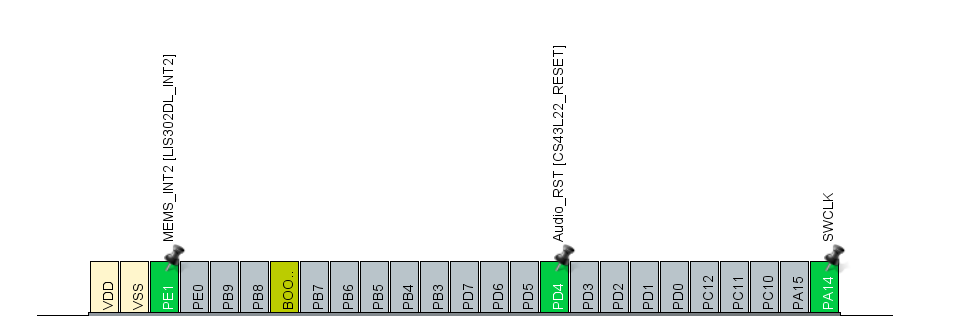
\includegraphics[angle=270, width=0.35\linewidth]{Maestro/pines1.png}
    \caption{Vista Pinout \& Configuration del Maestro: asignación de PB10/PB11 para USART3 y GPIO para RST/RTS/CTS.}
    \label{fig:ioc_pinout_maestro}
\end{figure}

\begin{figure}[H]
    \centering
    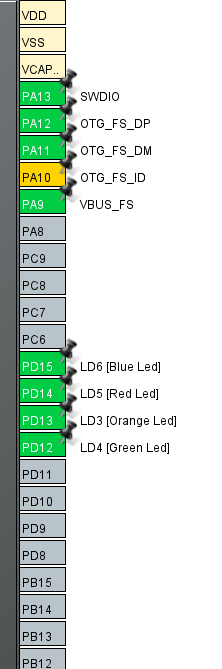
\includegraphics[width=0.25\linewidth]{Maestro/pines 2.png}
    \caption{Vista Pinout \& Configuration del Maestro: asignación de PB10/PB11 para USART3 y GPIO para RST/RTS/CTS.}
    \label{fig:ioc_pinout_maestro}
\end{figure}

\begin{figure}[H]
    \centering
    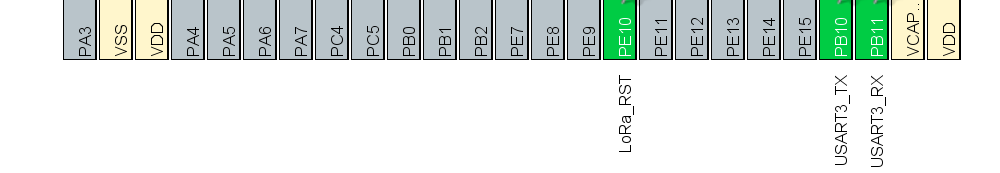
\includegraphics[angle=270,width=0.25\linewidth]{Maestro/pines3.png}
    \caption{Vista Pinout \& Configuration del Maestro: asignación de PB10/PB11 para USART3 y GPIO para RST/RTS/CTS.}
    \label{fig:ioc_pinout_maestro}
\end{figure}

\begin{figure}[H]
    \centering
    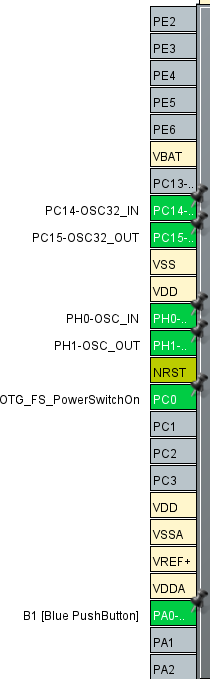
\includegraphics[width=0.25\linewidth]{Maestro/pines4.png}
    \caption{Vista Pinout \& Configuration del Maestro: asignación de PB10/PB11 para USART3 y GPIO para RST/RTS/CTS.}
    \label{fig:ioc_pinout_maestro}
\end{figure}


% ============================
\subsection{Configuración de periféricos (USART3)}
El RN2483 se comunica por UART a \textbf{57600\,bps}, \textbf{8N1}, sin control de flujo por hardware. En CubeMX:

\begin{enumerate}
    \item En \textbf{Pinout \& Configuration} $\rightarrow$ \textbf{Connectivity} $\rightarrow$ \textbf{USART3}, marca \textbf{Asynchronous}.
    \item En \textbf{Parameter Settings}:
    \begin{itemize}
        \item \textbf{Baud Rate}: \texttt{57600}
        \item \textbf{Word Length}: \texttt{8 Bits}
        \item \textbf{Parity}: \texttt{None}
        \item \textbf{Stop Bits}: \texttt{1}
        \item \textbf{Mode}: \texttt{TX and RX}
        \item \textbf{Hardware Flow Control}: \texttt{None} (RTS/CTS por GPIO)
        \item \textbf{OverSampling}: \texttt{16}
    \end{itemize}
\end{enumerate}


\begin{figure}[H]
    \centering
    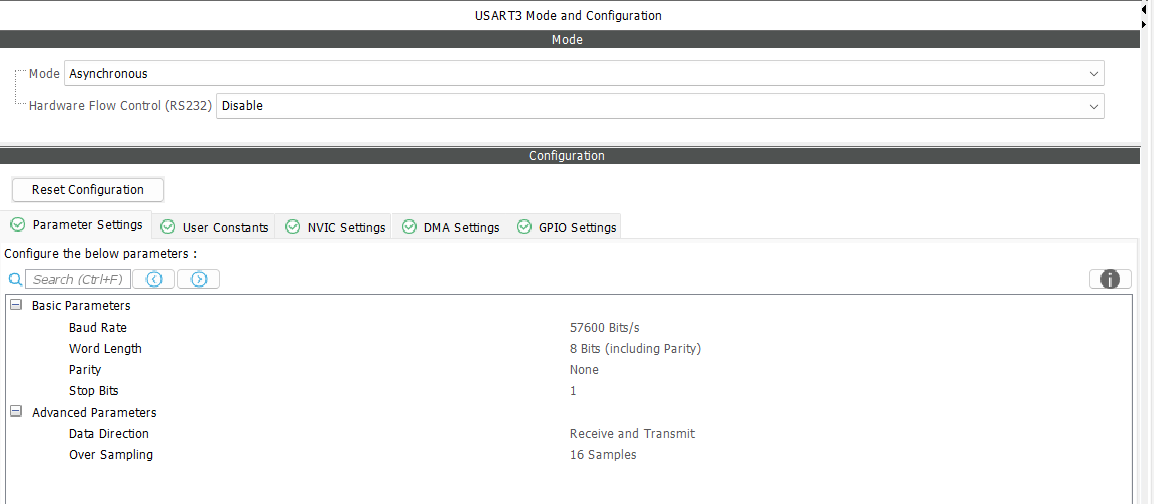
\includegraphics[width=0.85\linewidth]{Maestro/usart3.png}
    \caption{Parámetros de USART3 en CubeMX para el Maestro (57600\,bps, 8N1, sin flujo por hardware).}
    \label{fig:ioc_usart3_params_maestro}
\end{figure}

\subsection{Funciones para el uso del módulo LoRa como maestro}

En esta subsección estudiamos las rutinas que permiten inicializar, configurar y transmitir con el módulo \textbf{RN2483} desde el Maestro. Todas las funciones están escritas para trabajar con \textbf{USART3} (PB10/PB11) y con \textbf{RST} en PE10. La comunicación se realiza en modo \textit{radio} punto a punto (no LoRaWAN), enviando \textit{payloads} en formato \textbf{HEX ASCII} (por ejemplo, el dígito \texttt{'1'} se transmite como \texttt{"31"}).

\subsubsection{Pulso de reset al RN2483}
El pulso de reset garantiza un arranque limpio y que el RN2483 emita su banner de inicio. Tras el pulso, es normal que el módulo tarde decenas de milisegundos en quedar listo.

\newpage

\begin{lstlisting}[language=C, caption={Pulso de reset sobre RST (PE10)}, label={lst:lora_reset}]
static inline void LORA_Reset_Pulse(void)
{
  // RST PE10: Low 10 ms, luego High
  HAL_GPIO_WritePin(GPIOE, GPIO_PIN_10, GPIO_PIN_RESET);
  HAL_Delay(10);
  HAL_GPIO_WritePin(GPIOE, GPIO_PIN_10, GPIO_PIN_SET);
  HAL_Delay(100); // esperar banner de inicio
}
\end{lstlisting}


\begin{itemize}
  \item \texttt{GPIO\_PIN\_RESET} por 10\,ms fuerza el reinicio del RN2483.
  \item La espera de \texttt{100\,ms} da tiempo al módulo para inicializar su UART y banner de texto.
\end{itemize}

\subsubsection{Conversión a HEX ASCII (para radio tx)}
El comando \texttt{radio tx} del RN2483 exige que el \textit{payload} vaya en \textbf{HEX ASCII}. Por eso convertimos cada byte a dos caracteres HEX.

\begin{lstlisting}[language=C, caption={Conversión de un byte a dos dígitos HEX ASCII}, label={lst:u8_to_hex2}]
static void u8_to_hex2(uint8_t b, char out[3]) {
  const char *H = "0123456789ABCDEF";
  out[0] = H[(b >> 4) & 0x0F];
  out[1] = H[b & 0x0F];
  out[2] = '\0';
}
\end{lstlisting}

\noindent\textbf{Ejemplo:} \texttt{0x31} $\rightarrow$ \texttt{"31"}; el carácter \texttt{'1'} (ASCII 0x31) se envía como \texttt{"31"}.

\newpage
\subsubsection{Enviar y leer líneas por UART (polling)}
Trabajamos con funciones simples \textit{línea-a-línea} para transmitir comandos y leer respuestas hasta \texttt{\textbackslash n}, ignorando \texttt{\textbackslash r}.

\begin{lstlisting}[language=C, caption={Enviar una línea con terminador CR+LF}, label={lst:lora_sendline}]
static int LORA_SendLine(const char *line, uint32_t timeout_ms)
{
  char tx[128];
  int n = snprintf(tx, sizeof(tx), "%s\r\n", line);
  if (n <= 0) return -1;
  if (HAL_UART_Transmit(&huart3, (uint8_t*)tx, (uint16_t)n, timeout_ms) != HAL_OK) return -2;
  return 0;
}
\end{lstlisting}

\begin{lstlisting}[language=C, caption={Leer una línea hasta \textbackslash n con timeout}, label={lst:lora_readline}]
static int LORA_ReadLine(char *out, size_t out_sz, uint32_t timeout_ms)
{
  size_t idx = 0;
  uint8_t ch;
  uint32_t start = HAL_GetTick();
  while ((HAL_GetTick() - start) < timeout_ms && idx < (out_sz-1))
  {
    if (HAL_UART_Receive(&huart3, &ch, 1, 10) == HAL_OK)
    {
      if (ch == '\n') break;
      if (ch != '\r') out[idx++] = ch;
    }
  }
  out[idx] = '\0';
  return (idx > 0) ? (int)idx : -1;
}
\end{lstlisting}

\noindent\textbf{Claves didácticas:}
\begin{itemize}
  \item Siempre se envía \texttt{CR+LF} (\texttt{\textbackslash r\textbackslash n}) tras cada comando.
  \item \texttt{LORA\_ReadLine} usa una ventana total \texttt{timeout\_ms}, con lecturas de 10\,ms para no bloquear.
  \item Si retorna \texttt{-1}, no llegó respuesta en el tiempo dado (revisar cableado/baudios/reset/alimentación).
\end{itemize}

\subsubsection{Arranque y verificación del módulo}
Tras el \textit{reset}, solicitamos la versión con \texttt{sys get ver}. Si esta etapa falla, no seguimos con TX.

\begin{lstlisting}[language=C, caption={Boot y chequeo de versión del RN2483}, label={lst:lora_bootcheck}]
static int LORA_BootAndCheck(void)
{
  char line[128];

  LORA_Reset_Pulse();

  // Algunos RN2483 envian un banner tras reset; intenta leerlo sin bloquearte mucho
  LORA_ReadLine(line, sizeof(line), 300);

  if (LORA_SendLine("sys get ver", 200) != 0) return -1;
  if (LORA_ReadLine(line, sizeof(line), 500) < 0) return -2;

  // Aqui podrias validar prefijo "RN"
  return 0;
}
\end{lstlisting}

\noindent\textbf{Sugerencia práctica:} imprimir \texttt{line} por una UART de depuración o verlo en \textit{Live Expressions} para confirmar que contiene algo como \texttt{RN2483 1.0.X}.

\subsubsection{Transmisión básica en modo ``radio'' (punto a punto)}
El modo \textit{radio} funciona sin LoRaWAN y es ideal para pruebas P2P. Primero pausamos el stack MAC (\texttt{mac pause}), configuramos los parámetros físicos, y finalmente transmitimos.

\newpage

\begin{lstlisting}[language=C, caption={TX básico punto a punto con configuración LoRa}, label={lst:lora_radio_tx}]
static int LORA_RadioBasicTx(const char *hex_payload)
{
  char cmd[64], resp[64];

  LORA_SendLine("mac pause", 200);
  LORA_ReadLine(resp, sizeof(resp), 500);   // suele devolver "4294967295"

  // Config LoRa basica @433 MHz
  LORA_SendLine("radio set mod lora", 200);
  LORA_ReadLine(resp, sizeof(resp), 300);

  LORA_SendLine("radio set freq 433000000", 200);
  LORA_ReadLine(resp, sizeof(resp), 300);

  LORA_SendLine("radio set pwr 14", 200);
  LORA_ReadLine(resp, sizeof(resp), 300);

  LORA_SendLine("radio set sf sf7", 200);
  LORA_ReadLine(resp, sizeof(resp), 300);

  // BW correcto para LoRa (125/250/500)
  LORA_SendLine("radio set bw 125", 200);
  LORA_ReadLine(resp, sizeof(resp), 300);

  // Coding rate (4/5..4/8), CRC on, IQ invert off, preamble 8 (ajustables)
  LORA_SendLine("radio set cr 4/5", 200);
  LORA_ReadLine(resp, sizeof(resp), 300);

  LORA_SendLine("radio set crc on", 200);
  LORA_ReadLine(resp, sizeof(resp), 300);

  LORA_SendLine("radio set iqi off", 200);
  LORA_ReadLine(resp, sizeof(resp), 300);

  LORA_SendLine("radio set prlen 8", 200);
  LORA_ReadLine(resp, sizeof(resp), 300);

  // WDT 0 para evitar timeouts en radio
  LORA_SendLine("radio set wdt 0", 200);
  LORA_ReadLine(resp, sizeof(resp), 300);

  // TX
  snprintf(cmd, sizeof(cmd), "radio tx %s", hex_payload);
  if (LORA_SendLine(cmd, 500) != 0) return -1;

  if (LORA_ReadLine(resp, sizeof(resp), 500) < 0) return -2;   // esperado: "ok"
  if (LORA_ReadLine(resp, sizeof(resp), 2000) < 0) return -3;  // esperado: "radio_tx_ok"
  return 0;
}
\end{lstlisting}

\paragraph{Explicación parámetro por parámetro}
\begin{itemize}
  \item \texttt{mac pause}: deshabilita LoRaWAN y cede el control al modo \texttt{radio}. Devuelve un número (típicamente \texttt{4294967295}).
  \item \texttt{radio set mod lora}: define modulación LoRa (no FSK).
  \item \texttt{radio set freq \dots}: \textbf{frecuencia en Hz}. Para 433\,MHz: \texttt{433000000}. Para 868\,MHz: \texttt{868000000}.
  \item \texttt{radio set pwr 14}: potencia de TX en dBm (típico \texttt{2..14} según región/módulo).
  \item \texttt{radio set sf sf7}: \textbf{Spreading Factor} (\texttt{sf7} a \texttt{sf12}). Mayor SF $\Rightarrow$ mayor alcance y tiempo de aire.
  \item \texttt{radio set bw 125}: \textbf{Bandwidth} en kHz (\texttt{125}, \texttt{250}, \texttt{500}). Menor BW $\Rightarrow$ mayor sensibilidad.
  \item \texttt{radio set cr 4/5}: \textbf{Coding Rate} (\texttt{4/5} .. \texttt{4/8}). Mayor redundancia $\Rightarrow$ más robusto.
  \item \texttt{radio set crc on}: habilita CRC para detectar errores en payload.
  \item \texttt{radio set iqi off}: inversión de IQ; normalmente \texttt{off} para enlaces P2P estándar.
  \item \texttt{radio set prlen 8}: preámbulo; valores típicos \texttt{8..12}.
  \item \texttt{radio set wdt 0}: desactiva \textit{watchdog} interno de radio (evita abortos por tiempo).
\end{itemize}

\textbf{Cómo cambiar de 433\,MHz a 868\,MHz}

\begin{lstlisting}[language=C, caption={Frecuencia de operación}, label={lst:lora_freq}]
/* 433 MHz */
LORA_SendLine("radio set freq 433000000", 200);

/* 868 MHz */
LORA_SendLine("radio set freq 868000000", 200);
\end{lstlisting}

\noindent\textbf{Importante:} Maestro y Esclavo deben usar \textbf{exactamente los mismos} parámetros de \texttt{freq}, \texttt{sf}, \texttt{bw}, \texttt{cr}, \texttt{crc}, \texttt{iqi} y \texttt{prlen} para recibir correctamente.

\paragraph{Ajustes recomendados por escenario}
\begin{itemize}
  \item \textbf{Prueba de laboratorio}: \texttt{sf7}, \texttt{bw 125}, \texttt{pwr 10..14}, \texttt{prlen 8}.
  \item \textbf{Alcance medio} (paredes/obstáculos): subir a \texttt{sf9..sf10} y/o \texttt{pwr 14}.
  \item \textbf{Máximo alcance}: \texttt{sf12}, \texttt{bw 125}, \texttt{pwr 14} (mayor tiempo de aire).
\end{itemize}

\subsubsection{Integración en \texttt{main()} (fragmento inicial)}
En el \texttt{main} inicializamos periféricos y comprobamos el RN2483. Si \texttt{LORA\_BootAndCheck()} falla, encendemos un LED de error (o informamos por la consola).

\begin{lstlisting}[language=C, caption={Fragmento didáctico del main: boot + verificación}, label={lst:main_boot}]
/* USER CODE BEGIN 2 */
// Boot + version del LoRa
if (LORA_BootAndCheck() != 0) {
  // aqui puedes encender un LED o imprimir por otra UART para saber que fallo
}
/* USER CODE END 2 */
\end{lstlisting}

\paragraph{Checklist rápido antes de probar TX}
\begin{itemize}
  \item[$\Square$] USART3 a 57600\,bps (8N1) y cableado cruzado: \texttt{TX}\,$\rightarrow$\,\texttt{RX}, \texttt{RX}\,$\rightarrow$\,\texttt{TX}.
  \item[$\Square$] RST (PE10) configurado como salida; el pulso de reset funciona.
  \item[$\Square$] Alimentación y antena del RN2483 conectadas.
  \item[$\Square$] Mismo set de parámetros \texttt{radio set ...} en Maestro y Esclavo.
\end{itemize}

\subsubsection{Diagnóstico de respuestas típicas}
\begin{itemize}
  \item \textbf{Tras \texttt{radio tx}}: primero \texttt{ok}, luego \texttt{radio\_tx\_ok}. Si aparece \texttt{radio\_err}, revisar frecuencia/BW/SF o antena.
  \item \textbf{Sin respuesta}: revisar baudios (57600), pinout PB10/PB11 en AF7, masa común entre placa y módulo, y el pulso de \texttt{RST}.
  \item \textbf{Banner vacío}: ampliar el \texttt{HAL\_Delay(100)} tras \texttt{RST} a \texttt{200..400\,ms} en entornos ruidosos.
\end{itemize}

\subsection{Codigo y explicacion del main}

En esta parte dejamos listo el armazon del programa: inicializacion del HAL, reloj, GPIO, USB Host (opcional) y USART3. Tambien verificamos que el RN2483 responde antes de pasar al bucle principal (la logica del \texttt{while} se aborda en la siguiente subseccion).

\paragraph{Flujo general del \texttt{main}}
\begin{enumerate}
  \item \textbf{HAL\_Init()} y \textbf{SystemClock\_Config()} para preparar la MCU.
  \item \textbf{MX\_GPIO\_Init()} para RST/RTS/CTS y LEDs de la placa.
  \item \textbf{MX\_USB\_HOST\_Init()} (\emph{opcional} segun tu plantilla de proyecto).
  \item \textbf{MX\_USART3\_UART\_Init()} a 57600\,bps (8N1).
  \item \textbf{LORA\_BootAndCheck()} para resetear y consultar \texttt{sys get ver}.
  \item Si OK, encendemos LED verde; si falla, LED rojo.
\end{enumerate}
\newpage

\begin{lstlisting}[language=C, caption={Maestro: main antes del while (sin SPI ni TIM)}, label={lst:maestro_main_prewhile}]


int main(void)
{
  /* USER CODE BEGIN 1 */
  /* optional user init here */
  /* USER CODE END 1 */

  /* Reset of all peripherals, Initializes the Flash interface and the Systick. */
  HAL_Init();

  /* Configure the system clock */
  SystemClock_Config();

  /* Initialize all configured peripherals */
  MX_GPIO_Init();
  MX_USB_HOST_Init();      /* optional if your project uses USB Host */
  MX_USART3_UART_Init();

  /* USER CODE BEGIN 2 */
  /* turn off LEDs initially (PD12..PD15 on STM32F407G-DISC1) */
  HAL_GPIO_WritePin(GPIOD, GPIO_PIN_12|GPIO_PIN_13|GPIO_PIN_14|GPIO_PIN_15, GPIO_PIN_RESET);

  /* Boot + version check of RN2483 */
  if (LORA_BootAndCheck() == 0) {
    /* green LED = OK */
    HAL_GPIO_WritePin(GPIOD, GPIO_PIN_12, GPIO_PIN_SET);
  } else {
    /* red LED = FAIL */
    HAL_GPIO_WritePin(GPIOD, GPIO_PIN_14, GPIO_PIN_SET);
  }
  /* USER CODE END 2 */

 
}
\end{lstlisting}

\paragraph{Explicacion didactica, linea por linea (resumen)}
\begin{itemize}
  \item \texttt{HAL\_Init();} inicializa la capa HAL y el SysTick. Sin esto, los \texttt{HAL\_Delay()} no funcionan.
  \item \texttt{SystemClock\_Config();} define la fuente y multiplicadores del reloj. Mantener estable para evitar drift en UART.
  \item \texttt{MX\_GPIO\_Init();} configura: 
  \begin{itemize}
    \item \textbf{PE10} como salida para \texttt{RST} del RN2483.
    \item \textbf{PB12} como salida para \texttt{RTS} (software).
    \item \textbf{PE7} como entrada para \texttt{CTS} (software).
    \item LEDs \textbf{PD12..PD15} para diagnostico visual.
  \end{itemize}
  \item \texttt{MX\_USB\_HOST\_Init();} es opcional; si tu proyecto plantilla ya lo incluye, lo mantenemos.
  \item \texttt{MX\_USART3\_UART\_Init();} coloca la UART a 57600\,bps, 8N1, sin hardware flow control (coincide con RN2483).
  \item \texttt{LORA\_BootAndCheck();} hace \textit{reset} del modulo y envia \texttt{"sys get ver"}. Si responde, LED verde; si no, LED rojo.
\end{itemize}



\paragraph{Checklist rapido de esta etapa}
\begin{itemize}
  \item[$\square$] USART3 activo a 57600\,bps (AF7 en PB10/PB11).
  \item[$\square$] RST en PE10 funcionando (pulso bajo + retardo).
  \item[$\square$] LED verde enciende si hay respuesta del RN2483; rojo si falla.
\end{itemize}

\subsection{Codigo y explicacion del while}

El bucle principal realiza un envio periodico de un dato simple (un digito ASCII 0..9) al Esclavo. El payload se manda en \textbf{HEX ASCII} porque el comando \texttt{radio tx} del RN2483 lo exige. Por ejemplo, el caracter \texttt{'1'} (ASCII 0x31) se transmite como \texttt{"31"}.
\newpage

\begin{lstlisting}[language=C, caption={While del Maestro: envio periodico 0..9 en HEX ASCII}, label={lst:maestro_while}]
/* Infinite loop */
/* USER CODE BEGIN WHILE */
while (1)
{
  /* Mantener tareas de USB Host (si aplica en tu plantilla) */
  MX_USB_HOST_Process();

  /* Envio periodico cada 1000 ms */
  static uint8_t dig = 0;          // digito actual (0..9)
  static uint32_t t_tx = 0;
  const uint32_t TX_PERIOD_MS = 1000;

  if (HAL_GetTick() - t_tx >= TX_PERIOD_MS)
  {
    t_tx = HAL_GetTick();

    /* Convertir el digito '0'..'9' a su codigo ASCII y luego a HEX ASCII */
    char payload_hex[3];                              // 2 hex + terminador
    uint8_t ascii_digit = (uint8_t)('0' + dig);       // '0'..'9'
    u8_to_hex2(ascii_digit, payload_hex);             // ej. '1' -> "31"

    /* Transmitir por LoRa en modo radio (punto a punto) */
    int r = LORA_RadioBasicTx(payload_hex);           // envia "radio tx 30..39"
    if (r == 0) {
      /* LED verde = TX OK */
      HAL_GPIO_TogglePin(GPIOD, GPIO_PIN_12);
      /* apagar LED rojo por si estaba encendido */
      HAL_GPIO_WritePin(GPIOD, GPIO_PIN_14, GPIO_PIN_RESET);
    } else {
      /* LED rojo = fallo de TX */
      HAL_GPIO_WritePin(GPIOD, GPIO_PIN_14, GPIO_PIN_SET);
    }

    /* siguiente digito 0..9 */
    dig++;
    if (dig > 9) dig = 0;
  }
}
/* USER CODE END WHILE */
\end{lstlisting}

\paragraph{Que esta pasando paso a paso}
\begin{itemize}
  \item \textbf{Scheduler por millis}: se usa \texttt{HAL\_GetTick()} para disparar el envio cada \texttt{TX\_PERIOD\_MS}. Sin \texttt{HAL\_Delay} bloqueante, el bucle queda fluido.
  \item \textbf{Dato enviado}: el Maestro no manda el numero binario \texttt{0..9}, sino el \textbf{caracter ASCII} \texttt{'0'..'9'}. Ese byte ASCII se convierte a \textbf{HEX ASCII} con \texttt{u8\_to\_hex2} para ajustarse a \texttt{radio tx}.
  \item \textbf{Diagnostico visual}: si el envio termina en \texttt{radio\_tx\_ok}, se conmuta el LED verde (PD12). En error, se enciende el LED rojo (PD14).
  \item \textbf{Periodo de envio}: ajusta \texttt{TX\_PERIOD\_MS} (p.ej., 200 para 5 Hz o 5000 para 0.2 Hz).
\end{itemize}

\paragraph{Como enviar un byte arbitrario (p.ej., PWM 0..255)}
Si en lugar de un caracter \texttt{'0'..'9'} quieres mandar un valor de 0..255:
\begin{lstlisting}[language=C]
uint8_t pwm_byte = 127;     /* ejemplo */
char payload_hex[3];        /* "00".."FF" + '\0' */
u8_to_hex2(pwm_byte, payload_hex);
(int) LORA_RadioBasicTx(payload_hex);
\end{lstlisting}

\newpage

\paragraph{Como enviar dos bytes (p.ej., un valor de 10..bit)}
Concatena dos pares HEX:
\begin{lstlisting}[language=C]
uint16_t value = 1023;      /* ejemplo 10-bit */
char hex_hi[3], hex_lo[3], payload_hex[5]; /* "HHLL" + '\0' */
u8_to_hex2((uint8_t)(value >> 8), hex_hi);
u8_to_hex2((uint8_t)(value & 0xFF), hex_lo);
snprintf(payload_hex, sizeof(payload_hex), "%s%s", hex_hi, hex_lo);
/* Ej: 0x03FF -> "03FF" */
(int) LORA_RadioBasicTx(payload_hex);
\end{lstlisting}

\section{Analisis y explicacion del modulo Esclavo}

\subsection*{Que haremos en el Esclavo}
El Esclavo recibira por \textbf{LoRa RN2483} los datos enviados por el Maestro en modo \textit{radio} (punto a punto), decodificara el \textit{payload} en \textbf{HEX ASCII} (p. ej., "30".."39" representa '0'..'9') y los mostrara en la \textbf{OLED SSD1351}.

% ============================
\subsection{Configuracion e imagenes de los pines}

\paragraph{Pines del RN2483 (LoRa) en el Esclavo}
Para homogeneidad con el Maestro, mantenemos el mismo mapeo:
\begin{itemize}
    \item \textbf{RST} $\rightarrow$ \texttt{PE10}
    \item \textbf{RTS} $\rightarrow$ \texttt{PB12}
    \item \textbf{CTS} $\rightarrow$ \texttt{PE7}
    \item \textbf{TX}  $\rightarrow$ \texttt{PB11} (USART3\_TX)
    \item \textbf{RX}  $\rightarrow$ \texttt{PB10} (USART3\_RX)
\end{itemize}



\begin{table}[H]
\centering
\caption{Mapa de pines del Esclavo para LoRa RN2483}
\label{tab:pines_esclavo_lora}
\begin{tabular}{lll}
\toprule
\textbf{Senal RN2483} & \textbf{Pin STM32} & \textbf{Tipo / Uso} \\
\midrule
RST  & PE10 & GPIO salida (reset RN) \\
RTS  & PB12 & GPIO salida (flow control por software) \\
CTS  & PE7  & GPIO entrada (flow control por software) \\
TX   & PB11 & USART3\_TX (AF7) \\
RX   & PB10 & USART3\_RX (AF7) \\
\bottomrule
\end{tabular}
\end{table}

\paragraph{Pines de la OLED SSD1351 en el Esclavo}
Usaremos \textbf{SPI1} y las siguientes lineas de control:
\begin{itemize}
    \item \textbf{SPI1 SCK}  $\rightarrow$ \texttt{PB3}
    \item \textbf{SPI1 MISO} $\rightarrow$ \texttt{PB4}
    \item \textbf{SPI1 MOSI} $\rightarrow$ \texttt{PB5}
    \item \textbf{EN}        $\rightarrow$ \texttt{PD2} \quad (habilitacion del modulo)
    \item \textbf{RES}       $\rightarrow$ \texttt{PE4} \quad (reset OLED)
    \item \textbf{CS}        $\rightarrow$ \texttt{PE5} \quad (chip select)
    \item \textbf{RW}        $\rightarrow$ \texttt{PC5} \quad (read/write; normalmente en escritura)
    \item \textbf{D/C}       $\rightarrow$ \texttt{PB1} \quad (data/command)
\end{itemize}



\begin{table}[H]
\centering
\caption{Mapa de pines del Esclavo para OLED SSD1351 (SPI1)}
\label{tab:pines_esclavo_oled}
\begin{tabular}{lll}
\toprule
\textbf{Senal OLED} & \textbf{Pin STM32} & \textbf{Tipo / Uso} \\
\midrule
SCK   & PB3  & SPI1\_SCK \\
MISO  & PB4  & SPI1\_MISO \\
MOSI  & PB5  & SPI1\_MOSI \\
EN    & PD2  & GPIO salida (enable modulo) \\
RES   & PE4  & GPIO salida (reset OLED) \\
CS    & PE5  & GPIO salida (chip select) \\
RW    & PC5  & GPIO salida (modo escritura recomendado) \\
D/C   & PB1  & GPIO salida (seleccion dato/comando) \\
\bottomrule
\end{tabular}
\end{table}



\begin{figure}[H]
    \centering
    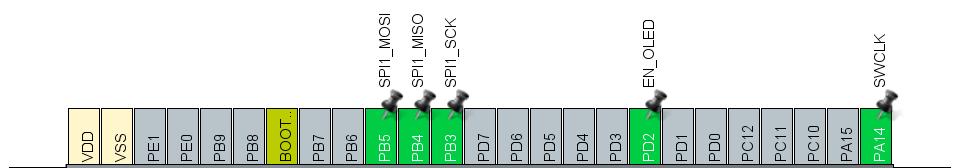
\includegraphics[angle=270, width=0.25\linewidth]{Esclavo/pines1.png}
    \caption{Esclavo: vista general de Pinout \& Configuration.}
    \label{fig:ioc_pinout_esclavo_overview}
\end{figure}

\begin{figure}[H]
    \centering
    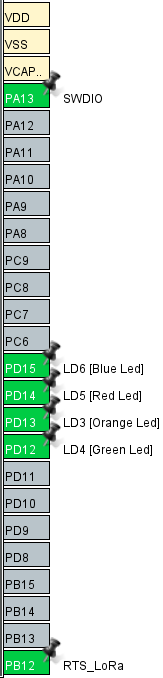
\includegraphics[width=0.25\linewidth]{Esclavo/pines2.png}
    \caption{Esclavo: vista general de Pinout \& Configuration.}
    \label{fig:ioc_pinout_esclavo_lora_af}
\end{figure}

\begin{figure}[H]
    \centering
    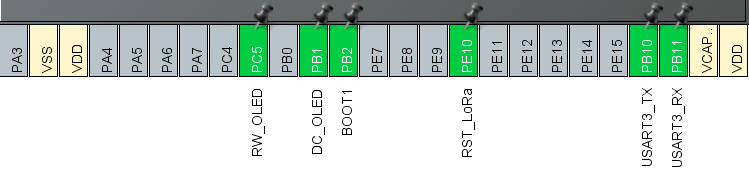
\includegraphics[angle=270, width=0.25\linewidth]{Esclavo/pines3.png}
    \caption{Esclavo: vista general de Pinout \& Configuration.}
    \label{fig:ioc_pinout_esclavo_spi1_af}
\end{figure}

\begin{figure}[H]
    \centering
    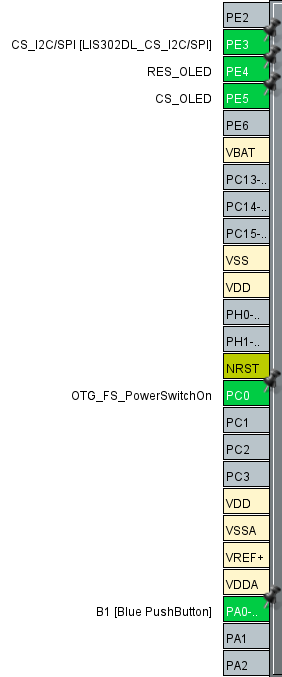
\includegraphics[width=0.45\linewidth]{Esclavo/pines4.png}
    \caption{Esclavo: vista general de Pinout \& Configuration.}
    \label{fig:ioc_pinout_esclavo_oled_gpio}
\end{figure}




\subsection{Configuracion de perifericos (USART3 y SPI1)}

\paragraph{USART3 (LoRa)}
El Esclavo usara \textbf{USART3} a \textbf{57600 bps}, \textbf{8N1}, \textbf{sin} control de flujo por hardware:
\begin{enumerate}
    \item \textbf{Pinout \& Configuration} $\rightarrow$ \textbf{Connectivity} $\rightarrow$ \textbf{USART3}: \textbf{Asynchronous}.
    \item \textbf{Parameter Settings}: \texttt{BaudRate=57600}, \texttt{WordLength=8B}, \texttt{Parity=None}, \texttt{StopBits=1}, \texttt{Mode=TX\&RX}, \texttt{HwFlowCtl=None}, \texttt{OverSampling=16}.
\end{enumerate}

\begin{figure}[H]
    \centering
    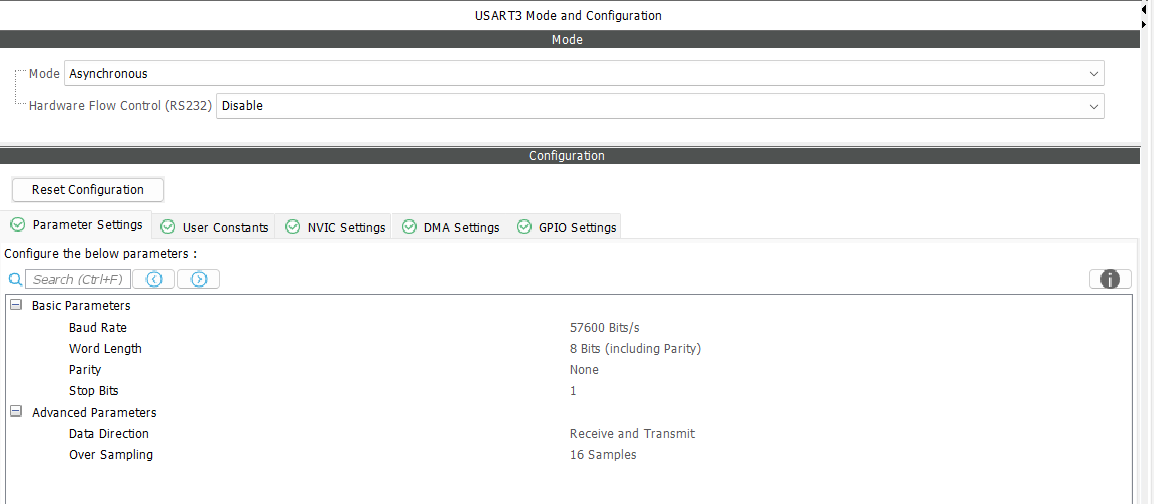
\includegraphics[width=0.85\linewidth]{Maestro/usart3.png}
    \caption{USART3 en CubeMX para Esclavo (57600 bps, 8N1, sin flujo por hardware).}
    \label{fig:ioc_usart3_params_esclavo}
\end{figure}

\paragraph{SPI1 (OLED)}
La OLED SSD1351 se comunica por \textbf{SPI1} como \textbf{Master, 8 bits}. Usa la configuracion que espera \texttt{ssd1351.c} (tu libreria). Un punto de partida comun es \textbf{SPI modo 0} (\texttt{CPOL=Low}, \texttt{CPHA=1Edge}). Si la imagen no aparece o muestra ruido, prueba \textbf{modo 3} (\texttt{CPOL=High}, \texttt{CPHA=2Edge}).

\begin{enumerate}
    \item \textbf{Pinout \& Configuration} $\rightarrow$ \textbf{Connectivity} $\rightarrow$ \textbf{SPI1}: \textbf{Full Duplex Master}.
    \item \textbf{Parameter Settings} (sugeridos):
    \begin{itemize}
        \item \textbf{Mode}: Master, \textbf{Direction}: 2Lines
        \item \textbf{Data Size}: 8 Bits, \textbf{First Bit}: MSB First
        \item \textbf{Clock Polarity}: Low, \textbf{Clock Phase}: 1 Edge  \quad(\textit{modo 0})
        \item \textbf{NSS}: Soft
        \item \textbf{BaudRate Prescaler}: 16 \quad(\(\approx\) 5.25 MHz con APB2 a 84 MHz)
        \item \textbf{TI Mode}: Disabled, \textbf{CRC}: Disabled
    \end{itemize}
\end{enumerate}

\begin{figure}[H]
    \centering
    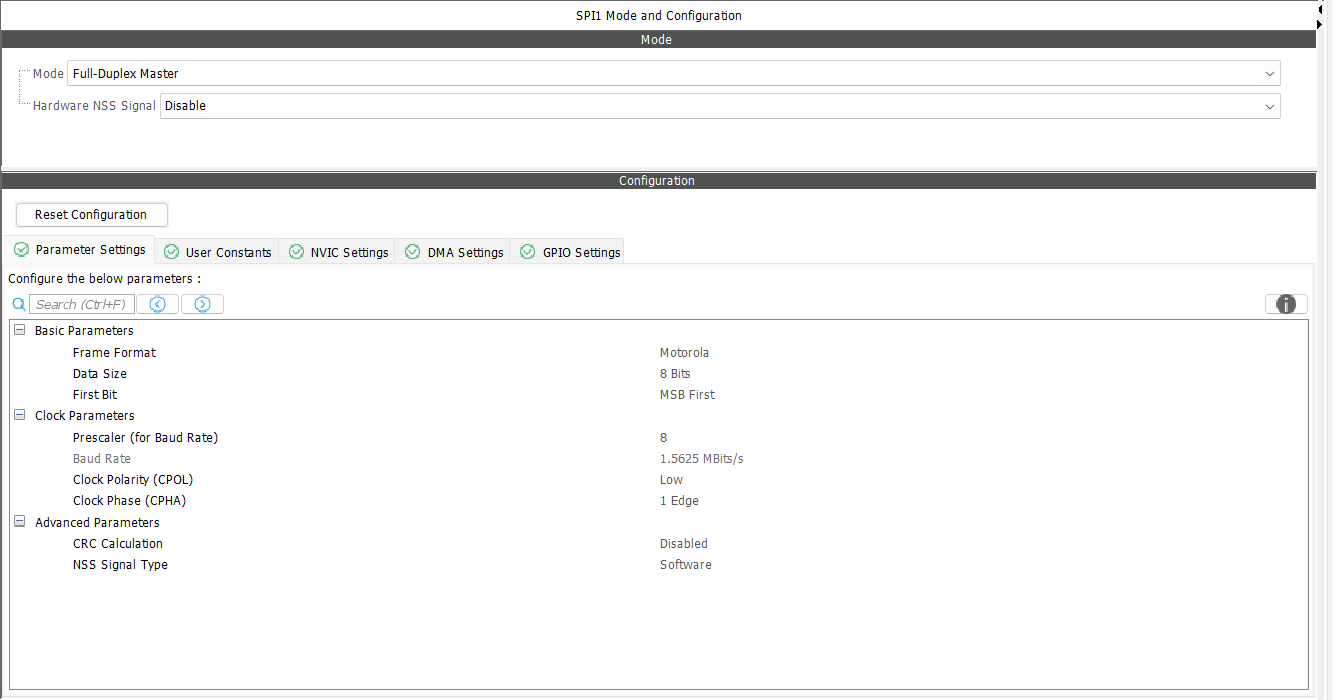
\includegraphics[width=0.85\linewidth]{Esclavo/spi1.png}
    \caption{SPI1 en CubeMX para Esclavo (SSD1351). Ajustar CPOL/CPHA segun libreria.}
    \label{fig:ioc_spi1_params_esclavo}
\end{figure}

\subsection{Funciones para la OLED (dentro de \texttt{main.c})}

En esta practica \textbf{reutilizamos la misma libreria} \texttt{ssd1351.c/.h} implementada en la practica anterior. 
Por lo tanto, \textbf{no reescribimos} la logica de bajo nivel (comandos, set column/row, protocolos, fuentes, etc.). 
Aqui solo dejamos claras las \textbf{exportaciones} necesarias y las \textbf{funciones minimas} en \texttt{main.c} para encender la pantalla, inicializarla y mostrar datos.

\paragraph{Exportaciones necesarias en \texttt{main.c}}
\begin{itemize}
  \item \texttt{\#include "ssd1351.h"} para acceder a \texttt{SSD1351\_Init()}, \texttt{SSD1351\_Clear()}, \texttt{SSD1351\_DrawText()}, etc.
  \item \texttt{extern SPI\_HandleTypeDef hspi1;} la libreria usa \texttt{hspi1} (SPI1) para transferencias.
  \item Asegurar que las \textbf{macros de pines} de la OLED usadas por la libreria (\texttt{OLED\_CS\_Pin}, \texttt{OLED\_DC\_Pin}, \texttt{OLED\_RES\_Pin}, \texttt{OLED\_EN\_Pin}, \texttt{OLED\_RW\_Pin}) \textbf{coinciden} con el mapeo de esta practica: 
  PB3=SCK, PB4=MISO, PB5=MOSI, PD2=EN, PE4=RES, PE5=CS, PC5=RW, PB1=DC.
\end{itemize}

\newpage

\begin{lstlisting}[language=C, caption={Includes y exports basicos para OLED en main.c}, label={lst:oled_exports}]
/* USER CODE BEGIN Includes */
#include "ssd1351.h"
#include <stdio.h>
#include <string.h>
#include <stdlib.h>
#include <ctype.h>
/* USER CODE END Includes */

/* USER CODE BEGIN PV */
extern SPI_HandleTypeDef hspi1;  /* usado por la libreria ssd1351 */
/* USER CODE END PV */
\end{lstlisting}

\paragraph{Secuencia de encendido + init (usar libreria anterior)}
La libreria ya realiza la inicializacion del controlador SSD1351. Antes de llamarla, recomendamos una secuencia simple de \textit{enable} y \textit{reset} desde GPIO para garantizar un arranque limpio.

\begin{lstlisting}[language=C, caption={Power-up basico y llamada a la libreria}, label={lst:oled_power_init}]
/* USER CODE BEGIN 2 */
/* habilitar modulo (si aplica en tu shield) */
HAL_GPIO_WritePin(OLED_EN_GPIO_Port, OLED_EN_Pin, GPIO_PIN_SET);

/* asegurarse de CS alto antes de configurar SPI */
HAL_GPIO_WritePin(OLED_CS_GPIO_Port, OLED_CS_Pin, GPIO_PIN_SET);

/* seleccionar escritura (si RW se usa) */
HAL_GPIO_WritePin(OLED_RW_GPIO_Port, OLED_RW_Pin, GPIO_PIN_RESET); /* write */

/* reset OLED */
HAL_GPIO_WritePin(OLED_RES_GPIO_Port, OLED_RES_Pin, GPIO_PIN_RESET);
HAL_Delay(10);
HAL_GPIO_WritePin(OLED_RES_GPIO_Port, OLED_RES_Pin, GPIO_PIN_SET);
HAL_Delay(100);

/* inicializacion via libreria de la practica anterior */
SSD1351_Init();
SSD1351_Clear();

/* mensaje de prueba */
SSD1351_DrawText(20, 0, "OLED OK", 0xFFFF, 0x0000, 2);
/* USER CODE END 2 */
\end{lstlisting}

\paragraph{Helpers minimos en \texttt{main.c} para esta practica}
Como ejemplo didactico, dejamos una funcion para \textbf{mostrar el ultimo digito recibido} (el Esclavo decodifica el payload y pasa el caracter que desea pintar). 
Todo el dibujo real lo hace la libreria (\texttt{DrawText}, colores RGB565, etc.).

\begin{lstlisting}[language=C, caption={Helper: mostrar un digito en la SSD1351}, label={lst:oled_show_digit}]
/* USER CODE BEGIN 0 */
static void OLED_ShowLastDigit(char c)
{
  /* etiqueta y valor en zona libre */
  SSD1351_DrawText(20, 66, "D:", 0xFFFF, 0x0000, 2);
  char s[2] = { c, '\0' };
  SSD1351_DrawText(50, 66, s, 0xFFE0, 0x0000, 2);
}
/* USER CODE END 0 */
\end{lstlisting}

\paragraph{Puntos a verificar para alinear libreria y hardware}
\begin{itemize}
  \item \textbf{SPI1}: PB3=SCK, PB4=MISO, PB5=MOSI en AF5. Parametros tipicos: 8-bit, Master, NSS=Soft, modo 0 (CPOL Low, CPHA 1Edge). 
        Si la imagen no aparece o sale ruido, probar modo 3 (CPOL High, CPHA 2Edge).
  \item \textbf{GPIO de control}: EN=PD2 (alto), RES=PE4 (pulso bajo), CS=PE5 (alto inactivo), RW=PC5 (low para escribir), DC=PB1 (0=cmd, 1=data).
  \item \textbf{Consistencia de macros}: que \texttt{ssd1351.c} use las mismas macros que definimos en esta guia.
  \item \textbf{Orden de llamadas}: primero GPIO (EN/RES/CS/RW), luego \texttt{MX\_SPI1\_Init()}, y finalmente \texttt{SSD1351\_Init()}.
\end{itemize}

Uso tipico desde \texttt{main()}
\begin{lstlisting}[language=C, caption={Uso sintetico en main(): init y mensaje}, label={lst:oled_use_main}]
/* USER CODE BEGIN 2 */
SSD1351_Init();
SSD1351_Clear();
SSD1351_DrawText(10, 10, "RX READY", 0x07E0, 0x0000, 1);
/* USER CODE END 2 */

/* ... en el while, cuando decodificas el payload ... */
OLED_ShowLastDigit('3');  /* ejemplo */
/* Tambien puedes imprimir diagnostico */
SSD1351_DrawText(0, 80, "RN: radio_rx 30", 0xFFFF, 0x0000, 1);
\end{lstlisting}

\subsection{Funciones para el uso del modulo LoRa como esclavo}

El Esclavo debe: (1) resetear el RN2483, (2) pausar el stack MAC, (3) aplicar la misma configuracion de radio que el Maestro (freq/SF/BW/CR/CRC/IQI/PRLEN), (4) entrar en modo escucha con \texttt{radio rx 0}, y (5) procesar eventos: \texttt{radio\_rx <hex>}, \texttt{radio\_err} o \texttt{busy}. 
Los helpers de UART 
LORA\_SendLine/LORA\_ReadLine
ya vistos se reutilizan tal cual.
\newpage

\textbf{Reset del RN2483 (GPIO PE10)}
\begin{lstlisting}[language=C, caption={Pulso de reset al RN2483}, label={lst:lora_rst_slave}]
static inline void LORA_Reset_Pulse(void)
{
  HAL_GPIO_WritePin(LORA_RST_GPIO_Port, LORA_RST_Pin, GPIO_PIN_RESET);
  HAL_Delay(10);
  HAL_GPIO_WritePin(LORA_RST_GPIO_Port, LORA_RST_Pin, GPIO_PIN_SET);
  HAL_Delay(300); /* tiempo para banner y UART lista */
}
\end{lstlisting}

\paragraph{Aplicar configuracion PHY por defecto (parametros de radio)}
La siguiente rutina aplica un set solido (igual al Maestro), dejando la \textbf{frecuencia} como argumento para que puedas conmutar entre 433 MHz y 868 MHz con una sola linea.

\begin{lstlisting}[language=C, caption={Configurar PHY LoRa basica para Esclavo}, label={lst:lora_apply_phy}]
static int LORA_ApplyDefaultPhy(uint32_t freq_hz)
{
  char resp[96], cmd[48];

  /* ceder control al modo radio (no LoRaWAN) */
  LORA_SendLine("mac pause", 200);
  LORA_ReadLine(resp, sizeof(resp), 500); /* tipico: 4294967295 */

  /* mod LoRa y parametros base */
  LORA_SendLine("radio set mod lora", 200);   LORA_ReadLine(resp, sizeof(resp), 300);

  snprintf(cmd, sizeof(cmd), "radio set freq %lu", (unsigned long)freq_hz);
  LORA_SendLine(cmd, 200);                    LORA_ReadLine(resp, sizeof(resp), 300);

  LORA_SendLine("radio set pwr 14", 200);     LORA_ReadLine(resp, sizeof(resp), 300);
  LORA_SendLine("radio set sf sf7", 200);     LORA_ReadLine(resp, sizeof(resp), 300);
  LORA_SendLine("radio set bw 125", 200);     LORA_ReadLine(resp, sizeof(resp), 300);
  LORA_SendLine("radio set cr 4/5", 200);     LORA_ReadLine(resp, sizeof(resp), 300);
  LORA_SendLine("radio set crc on", 200);     LORA_ReadLine(resp, sizeof(resp), 300);
  LORA_SendLine("radio set iqi off", 200);    LORA_ReadLine(resp, sizeof(resp), 300);
  LORA_SendLine("radio set prlen 8", 200);    LORA_ReadLine(resp, sizeof(resp), 300);
  LORA_SendLine("radio set wdt 0", 200);      LORA_ReadLine(resp, sizeof(resp), 300);

  return 0;
}
\end{lstlisting}

\textbf{Entrar en escucha continua (\texttt{radio rx 0})}
\begin{lstlisting}[language=C, caption={Inicializar y quedar escuchando}, label={lst:lora_init_listen}]
static int LORA_InitAndListen(uint32_t freq_hz)
{
  char resp[96];

  LORA_Reset_Pulse();                             /* reset fisico */
  LORA_SendLine("sys get ver", 300);              /* opcional: banner/version */
  LORA_ReadLine(resp, sizeof(resp), 1000);        /* no critico si no llega */

  if (LORA_ApplyDefaultPhy(freq_hz) != 0) return -1;

  if (LORA_SendLine("radio rx 0", 200) != 0) return -2;
  if (LORA_ReadLine(resp, sizeof(resp), 500) < 0) return -3; /* "ok" */
  HAL_Delay(20); /* evita "busy" inmediato */
  return 0;
}

/* atajos comodos */
static inline int LORA_InitAndListen_433(void) { return LORA_InitAndListen(433000000UL); }
static inline int LORA_InitAndListen_868(void) { return LORA_InitAndListen(868000000UL); }
\end{lstlisting}

\paragraph{Rearmar la recepcion tras cada evento}
El RN2483 requiere rearmar \texttt{radio rx 0} para seguir escuchando despues de cada evento (rx, err, busy).

\begin{lstlisting}[language=C, caption={Rearmar el receptor}, label={lst:lora_rearm_rx}]
static void LORA_RearmRx(void)
{
  char resp[32];
  LORA_SendLine("radio rx 0", 200);
  LORA_ReadLine(resp, sizeof(resp), 500); /* "ok" */
  HAL_Delay(20);
}
\end{lstlisting}

\paragraph{Decodificar el primer byte del payload (HEX ASCII)}
Los payloads del Maestro se envian en HEX ASCII (p. ej., '0' -> "30"). Esta funcion intenta extraer el \textbf{primer byte} del mensaje \texttt{radio\_rx <hex>}.

\begin{lstlisting}[language=C, caption={HEX ASCII -> byte (primer par)}, label={lst:hex2_to_u8}]
static int hex2_to_u8(const char *h, uint8_t *out)
{
  uint8_t v = 0;
  for (int i = 0; i < 2; i++) {
    char c = h[i];
    uint8_t d;
    if      (c >= '0' && c <= '9') d = (uint8_t)(c - '0');
    else if (c >= 'A' && c <= 'F') d = (uint8_t)(10 + (c - 'A'));
    else if (c >= 'a' && c <= 'f') d = (uint8_t)(10 + (c - 'a'));
    else return -1;
    v = (uint8_t)((v << 4) | d);
  }
  *out = v;
  return 0;
}
\end{lstlisting}

\newpage

\begin{lstlisting}[language=C, caption={Intentar decodificar el primer byte de "radio_rx ..." }, label={lst:lora_trydecode}]
static int LORA_TryDecodeFirstByte(const char *line, uint8_t *out_byte)
{
  /* espera "radio_rx <hex...>" */
  if (strncmp(line, "radio_rx ", 9) != 0) return 0; /* no es un paquete */

  const char *p = line + 9;
  while (*p == ' ') p++;             /* saltar espacios */
  if (!isxdigit((unsigned char)p[0]) || !isxdigit((unsigned char)p[1])) return -1;

  return hex2_to_u8(p, out_byte);    /* devuelve 0 si OK */
}
\end{lstlisting}

\paragraph{Poll no bloqueante: leer una linea y manejar eventos}
Este helper lee una linea del RN (con timeout corto) y, si hay paquete, \textbf{devuelve 1 y el byte decodificado}. Si no hay nada, devuelve \textbf{0}. En errores, \textbf{-1}. 
La rearmada de RX se hace internamente.

\begin{lstlisting}[language=C, caption={Poll y manejo de eventos LoRa en Esclavo}, label={lst:lora_poll_handle}]
static int LORA_PollAndGetByte(uint8_t *out_byte, uint32_t read_timeout_ms)
{
  char line[96];
  int n = LORA_ReadLine(line, sizeof(line), read_timeout_ms);
  if (n <= 0) return 0;       /* no hubo linea en este ciclo */

  /* opcional: aqui puedes dibujar 'line' en OLED para diagnostico */

  if (!strcmp(line, "radio_err") || !strcmp(line, "busy")) {
    LORA_RearmRx();
    return 0;
  }

  uint8_t b;
  int r = LORA_TryDecodeFirstByte(line, &b);
  if (r == 0) {
    /* paquete valido: rearmar y devolver el byte */
    LORA_RearmRx();
    *out_byte = b;
    return 1;
  } else if (r < 0) {
    /* linea "radio_rx ..." pero mal formada: rearmar */
    LORA_RearmRx();
    return -1;
  }

  /* otra linea informativa; no es paquete de datos */
  return 0;
}
\end{lstlisting}

\paragraph{Como elegir la frecuencia (433 vs 868 MHz)}
El Esclavo debe \textbf{igualar} la PHY del Maestro:
\begin{lstlisting}[language=C, caption={Elegir banda al iniciar}, label={lst:lora_band_select}]
/* 433 MHz */
if (LORA_InitAndListen_433() != 0) { /* manejo de error */ }

/* 868 MHz */
// if (LORA_InitAndListen_868() != 0) { /* manejo de error */ }
\end{lstlisting}

\subsection{Codigo y explicacion del main (Esclavo)}

En el \texttt{main()} inicializamos la MCU, GPIO, USART3 y SPI1; encendemos e inicializamos la \textbf{OLED SSD1351} con la libreria ya usada en la practica anterior; y dejamos el \textbf{RN2483} escuchando con \texttt{radio rx 0} (banda seleccionable 433/868 MHz). El bucle \texttt{while} se desarrolla en la siguiente subseccion.

\paragraph{Flujo general}
\begin{enumerate}
  \item \textbf{HAL\_Init()} y \textbf{SystemClock\_Config()}.
  \item \textbf{MX\_GPIO\_Init()} para LoRa (RST/RTS/CTS), OLED (EN/RES/CS/RW/DC) y LEDs.
  \item \textbf{MX\_USART3\_UART\_Init()} a 57600 bps (8N1, sin HW flow).
  \item \textbf{MX\_SPI1\_Init()} (modo master, 8 bits) para la OLED.
  \item \textbf{OLED power-up} (EN/RES/CS/RW) y \textbf{SSD1351\_Init()} de la libreria.
  \item \textbf{LoRa Init \& Listen} con misma PHY que el Maestro.
\end{enumerate}

\begin{lstlisting}[language=C, caption={Esclavo: main antes del while (OLED + LoRa)}, label={lst:esclavo_main_prewhile}]

int main(void)
{
  /* USER CODE BEGIN 1 */
  /* user pre-init (opcional) */
  /* USER CODE END 1 */

  HAL_Init();
  SystemClock_Config();

  MX_GPIO_Init();
  MX_USART3_UART_Init();
  MX_SPI1_Init();

  /* USER CODE BEGIN 2 */
  /* apagar LEDs inicialmente */
  HAL_GPIO_WritePin(GPIOD, GPIO_PIN_12|GPIO_PIN_13|GPIO_PIN_14|GPIO_PIN_15, GPIO_PIN_RESET);

  /* --- OLED power-up + init (reutiliza tu libreria ssd1351) --- */
  HAL_GPIO_WritePin(OLED_EN_GPIO_Port,  OLED_EN_Pin,  GPIO_PIN_SET);    /* enable */
  HAL_GPIO_WritePin(OLED_CS_GPIO_Port,  OLED_CS_Pin,  GPIO_PIN_SET);    /* CS high idle */
  HAL_GPIO_WritePin(OLED_RW_GPIO_Port,  OLED_RW_Pin,  GPIO_PIN_RESET);  /* write */
  HAL_GPIO_WritePin(OLED_RES_GPIO_Port, OLED_RES_Pin, GPIO_PIN_RESET);  /* reset */
  HAL_Delay(10);
  HAL_GPIO_WritePin(OLED_RES_GPIO_Port, OLED_RES_Pin, GPIO_PIN_SET);
  HAL_Delay(100);

  SSD1351_Init();               /* libreria de la practica anterior */
  SSD1351_Clear();
  SSD1351_DrawText(10, 0,  "OLED OK",  0xFFFF, 0x0000, 1);
  SSD1351_DrawText(10, 16, "LoRa RX...",0x07E0, 0x0000, 1);

  /* --- LoRa: inicializar y quedar escuchando --- */
  /* Elige banda segun tu prueba: 433 MHz o 868 MHz.
     Asegurate de que el Maestro usa la misma configuracion. */

  if (LORA_InitAndListen_433() == 0) {
    SSD1351_DrawText(10, 32, "LoRa RX OK", 0x07E0, 0x0000, 1);
    HAL_GPIO_WritePin(GPIOD, GPIO_PIN_12, GPIO_PIN_SET);  /* LED verde */
  } else {
    SSD1351_DrawText(10, 32, "LoRa FAIL",  0xF800, 0x0000, 1);
    HAL_GPIO_WritePin(GPIOD, GPIO_PIN_14, GPIO_PIN_SET);  /* LED rojo */
    /* puedes quedarte aqui o reintentar mas adelante */
  }
  /* USER CODE END 2 */

  /* Infinite loop */
  /* USER CODE BEGIN WHILE */

}
\end{lstlisting}

\paragraph{Explicacion didactica (resumen)}
\begin{itemize}
  \item \textbf{SPI1 (OLED)}: PB3=SCK, PB4=MISO, PB5=MOSI (AF5). NSS=Soft. Modo sugerido: 0 (CPOL Low, CPHA 1Edge); si ves ruido, probar modo 3.
  \item \textbf{GPIO OLED}: EN=PD2 (alto), RES=PE4 (pulso bajo), CS=PE5 (alto inactivo), RW=PC5 (low para escribir), DC=PB1 (0=cmd, 1=data).
  \item \textbf{USART3 (LoRa)}: PB10=RX, PB11=TX (AF7), 57600 bps, 8N1, sin HW flow. RST=PE10 con pulso de 10 ms + 300 ms de espera.
  \item \textbf{Init LoRa}: se pausa MAC (\texttt{mac pause}), se aplica PHY igual al Maestro (\texttt{freq/sf/bw/cr/crc/iqi/prlen}) y se arma \texttt{radio rx 0}.
\end{itemize}

\textbf{Cambiar rapidamente de 433 a 868 MHz}
\begin{lstlisting}[language=C]
/* 433 MHz por defecto */
if (LORA_InitAndListen_433() != 0) { /* manejo de error */ }

/* Para 868 MHz, usa esto en su lugar */
// if (LORA_InitAndListen_868() != 0) { /* manejo de error */ }
\end{lstlisting}

\subsection{Codigo y explicacion del while (Esclavo)}

El bucle principal consulta periodicamente al RN2483 sin bloquear, decodifica el \textit{payload} (primer byte en HEX ASCII) y actualiza la OLED. 
Si llega un paquete valido, parpadea el LED verde; si hay una linea mal formada, dejamos encendido el LED rojo como alerta.

\begin{lstlisting}[language=C, caption={While del Esclavo: recepcion, decodificacion y OLED}, label={lst:esclavo_while}]
/* Infinite loop */
/* USER CODE BEGIN WHILE */
while (1)
{
  /* Tiempo maximo de espera por linea en cada iteracion (ms) */
  const uint32_t READ_TIMEOUT_MS = 1000;

  uint8_t b;
  int got = LORA_PollAndGetByte(&b, READ_TIMEOUT_MS);

  if (got == 1) {
    /* Tenemos un byte decodificado del primer par HEX ("30".."39" -> '0'..'9') */
    char to_show;
    if (b >= '0' && b <= '9') {
      to_show = (char)b;               /* Maestro envia ASCII '0'..'9' */
    } else if (b <= 9) {
      to_show = (char)('0' + b);       /* soporte 00..09 crudo */
    } else {
      to_show = '.';
    }

    /* Mostrar en la OLED (helper de la subseccion OLED) */
    OLED_ShowLastDigit(to_show);

    /* Feedback visual: LED verde = RX OK */
    HAL_GPIO_TogglePin(GPIOD, GPIO_PIN_12);
    /* Asegurar LED rojo apagado cuando hay exito */
    HAL_GPIO_WritePin(GPIOD, GPIO_PIN_14, GPIO_PIN_RESET);
  }
  else if (got < 0) {
    /* Linea "radio_rx ..." pero mal formada (ya rearmamos RX) */
    HAL_GPIO_WritePin(GPIOD, GPIO_PIN_14, GPIO_PIN_SET);  /* LED rojo = alerta */
  }

  /* Aqui puedes incluir otras tareas no bloqueantes si las necesitas */
}
/* USER CODE END WHILE */
\end{lstlisting}

\paragraph{Que esta pasando}
\begin{itemize}
  \item \textbf{Lectura no bloqueante:} \texttt{LORA\_PollAndGetByte()} usa \texttt{LORA\_ReadLine()} con un timeout corto (1 s por vuelta). 
        Si no hay nada, devuelve 0 y el while sigue fluido.
  \item \textbf{Decodificacion HEX:} del mensaje \texttt{radio\_rx <hex...>} tomamos solo el \textbf{primer par HEX} y lo convertimos a byte. 
        Si el Maestro envia ASCII \texttt{'0'..'9'}, veras los digitos en la OLED.
  \item \textbf{Rearmado automatico:} despues de cada evento (rx/err/busy), el helper rearma internamente \texttt{radio rx 0}.
  \item \textbf{Diagnostico por LEDs:} verde (\texttt{PD12}) indica recepcion correcta; rojo (\texttt{PD14}) marca linea mal formada.
\end{itemize}

\paragraph{Prueba rapida}
\begin{enumerate}
  \item En el Maestro, confirma que estas enviando \texttt{"30".."39"} (ASCII de \texttt{'0'..'9'} en HEX).
  \item En el Esclavo, deberias ver el digito recibido en la OLED y el LED verde parpadear cada paquete.
  \item Si no recibes nada: revisa que \texttt{freq/sf/bw/cr/crc/iqi/prlen} coincidan, antena conectada, y que el Maestro no este demasiado cerca (saturacion).
\end{enumerate}

\section{Resultados}

En esta sección se presentan evidencias de funcionamiento y métricas simples del enlace Maestro–Esclavo usando \textbf{LoRa RN2483} en modo \textit{radio} (punto a punto). El Maestro transmite un dígito ASCII (\texttt{'0'..'9'}) cada 1\,s; el Esclavo recibe, decodifica (\textit{HEX ASCII}) y muestra el carácter en la \textbf{OLED SSD1351}. Se comparan además ambas bandas de operación (\textbf{433\,MHz} y \textbf{868\,MHz}).

\subsection{Imágenes del funcionamiento}

\begin{figure}[H]
  \centering
  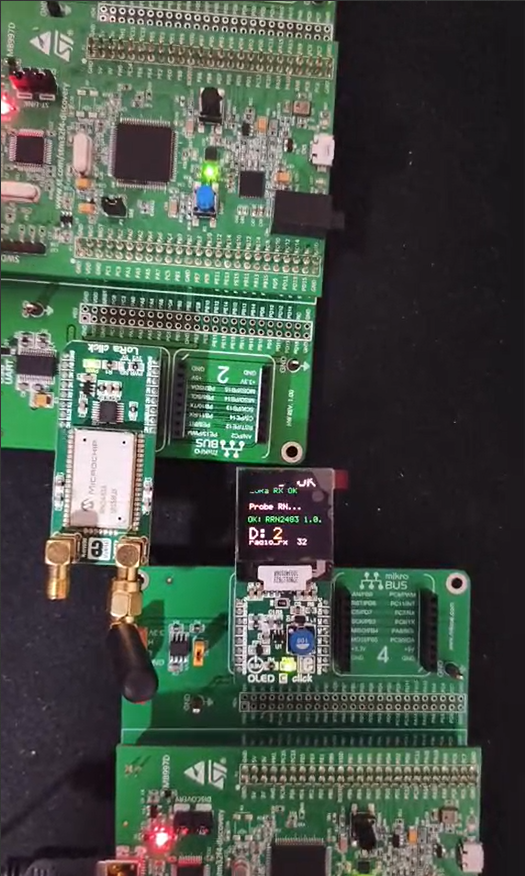
\includegraphics[width=0.6\linewidth]{Resultados/result1.png}
  \caption{Esclavo recibiendo: OLED mostrando el dígito decodificado (ej. ‘7’) y mensaje “LoRa RX OK”.}
  \label{fig:esclavo_rx}
\end{figure}



\subsection{Diferencias entre frecuencias (433\,MHz vs 868\,MHz)}

\paragraph{Penetración y pérdidas}
A igual distancia, la banda de 433\,MHz sufre \textbf{menor pérdida en espacio libre} que 868\,MHz (por la dependencia con la frecuencia). 
Usando la fórmula de path loss en espacio libre (FSPL, dB): 
\[
\mathrm{FSPL} = 32.44 + 20\log_{10}(f_{\mathrm{MHz}}) + 20\log_{10}(d_{\mathrm{km}})
\]
se tienen ejemplos didácticos:

\begin{table}[H]
\centering
\caption{FSPL teórica comparada (referencia)}
\label{tab:fspl}
\begin{tabular}{lccc}
\toprule
\textbf{Distancia} & \textbf{433\,MHz (dB)} & \textbf{868\,MHz (dB)} & \textbf{Δ (868-433)} \\
\midrule
10\,m  & 45.17 & 51.21 & \(\approx 6.0\) \\
50\,m  & 59.15 & 65.19 & \(\approx 6.0\) \\
100\,m & 65.17 & 71.21 & \(\approx 6.0\) \\
\bottomrule
\end{tabular}
\end{table}

\noindent
Esto explica que, en general, \textbf{433\,MHz} tiende a comportarse mejor en interiores u obstáculos (mayor longitud de onda, mejor difracción/penetración). 
Por su parte, \textbf{868\,MHz} usa antenas más cortas y, combinado con BW amplias y SF bajos, puede ofrecer menor \textit{time-on-air} (menor latencia) en escenarios de corto alcance.

\paragraph{Tamaño de antena (aprox. cuarto de onda)}
\[
\lambda = \frac{c}{f} \Rightarrow \lambda_{433}\approx 0.693\,\mathrm{m} \ (\lambda/4\approx 17.3\,\mathrm{cm}),\quad 
\lambda_{868}\approx 0.346\,\mathrm{m} \ (\lambda/4\approx 8.6\,\mathrm{cm})
\]
Antenas más cortas en 868\,MHz son prácticas para montajes compactos; 433\,MHz favorece enlaces más robustos con antenas algo más largas.

\paragraph{Parámetros físicos (SF/BW/CR) y ToA}
Con BW=125\,kHz y CR=4/5, el \textbf{tiempo en aire} para un \textbf{payload de 1\,byte} es, teóricamente:
\begin{itemize}
  \item SF7: \(\approx 25.9\,\mathrm{ms}\)
  \item SF9: \(\approx 103.4\,\mathrm{ms}\)
  \item SF12: \(\approx 827.4\,\mathrm{ms}\)
\end{itemize}
Reducir SF (p.ej., SF7) y/o aumentar BW (p.ej., 250/500\,kHz) disminuye el ToA y la latencia, a costa de alcance/robustez. 
\textbf{Maestro y Esclavo deben tener la misma PHY} (freq/SF/BW/CR/CRC/IQ/PRLEN).











\end{document}
